\begin{figure}[htbp]

\begin{center}
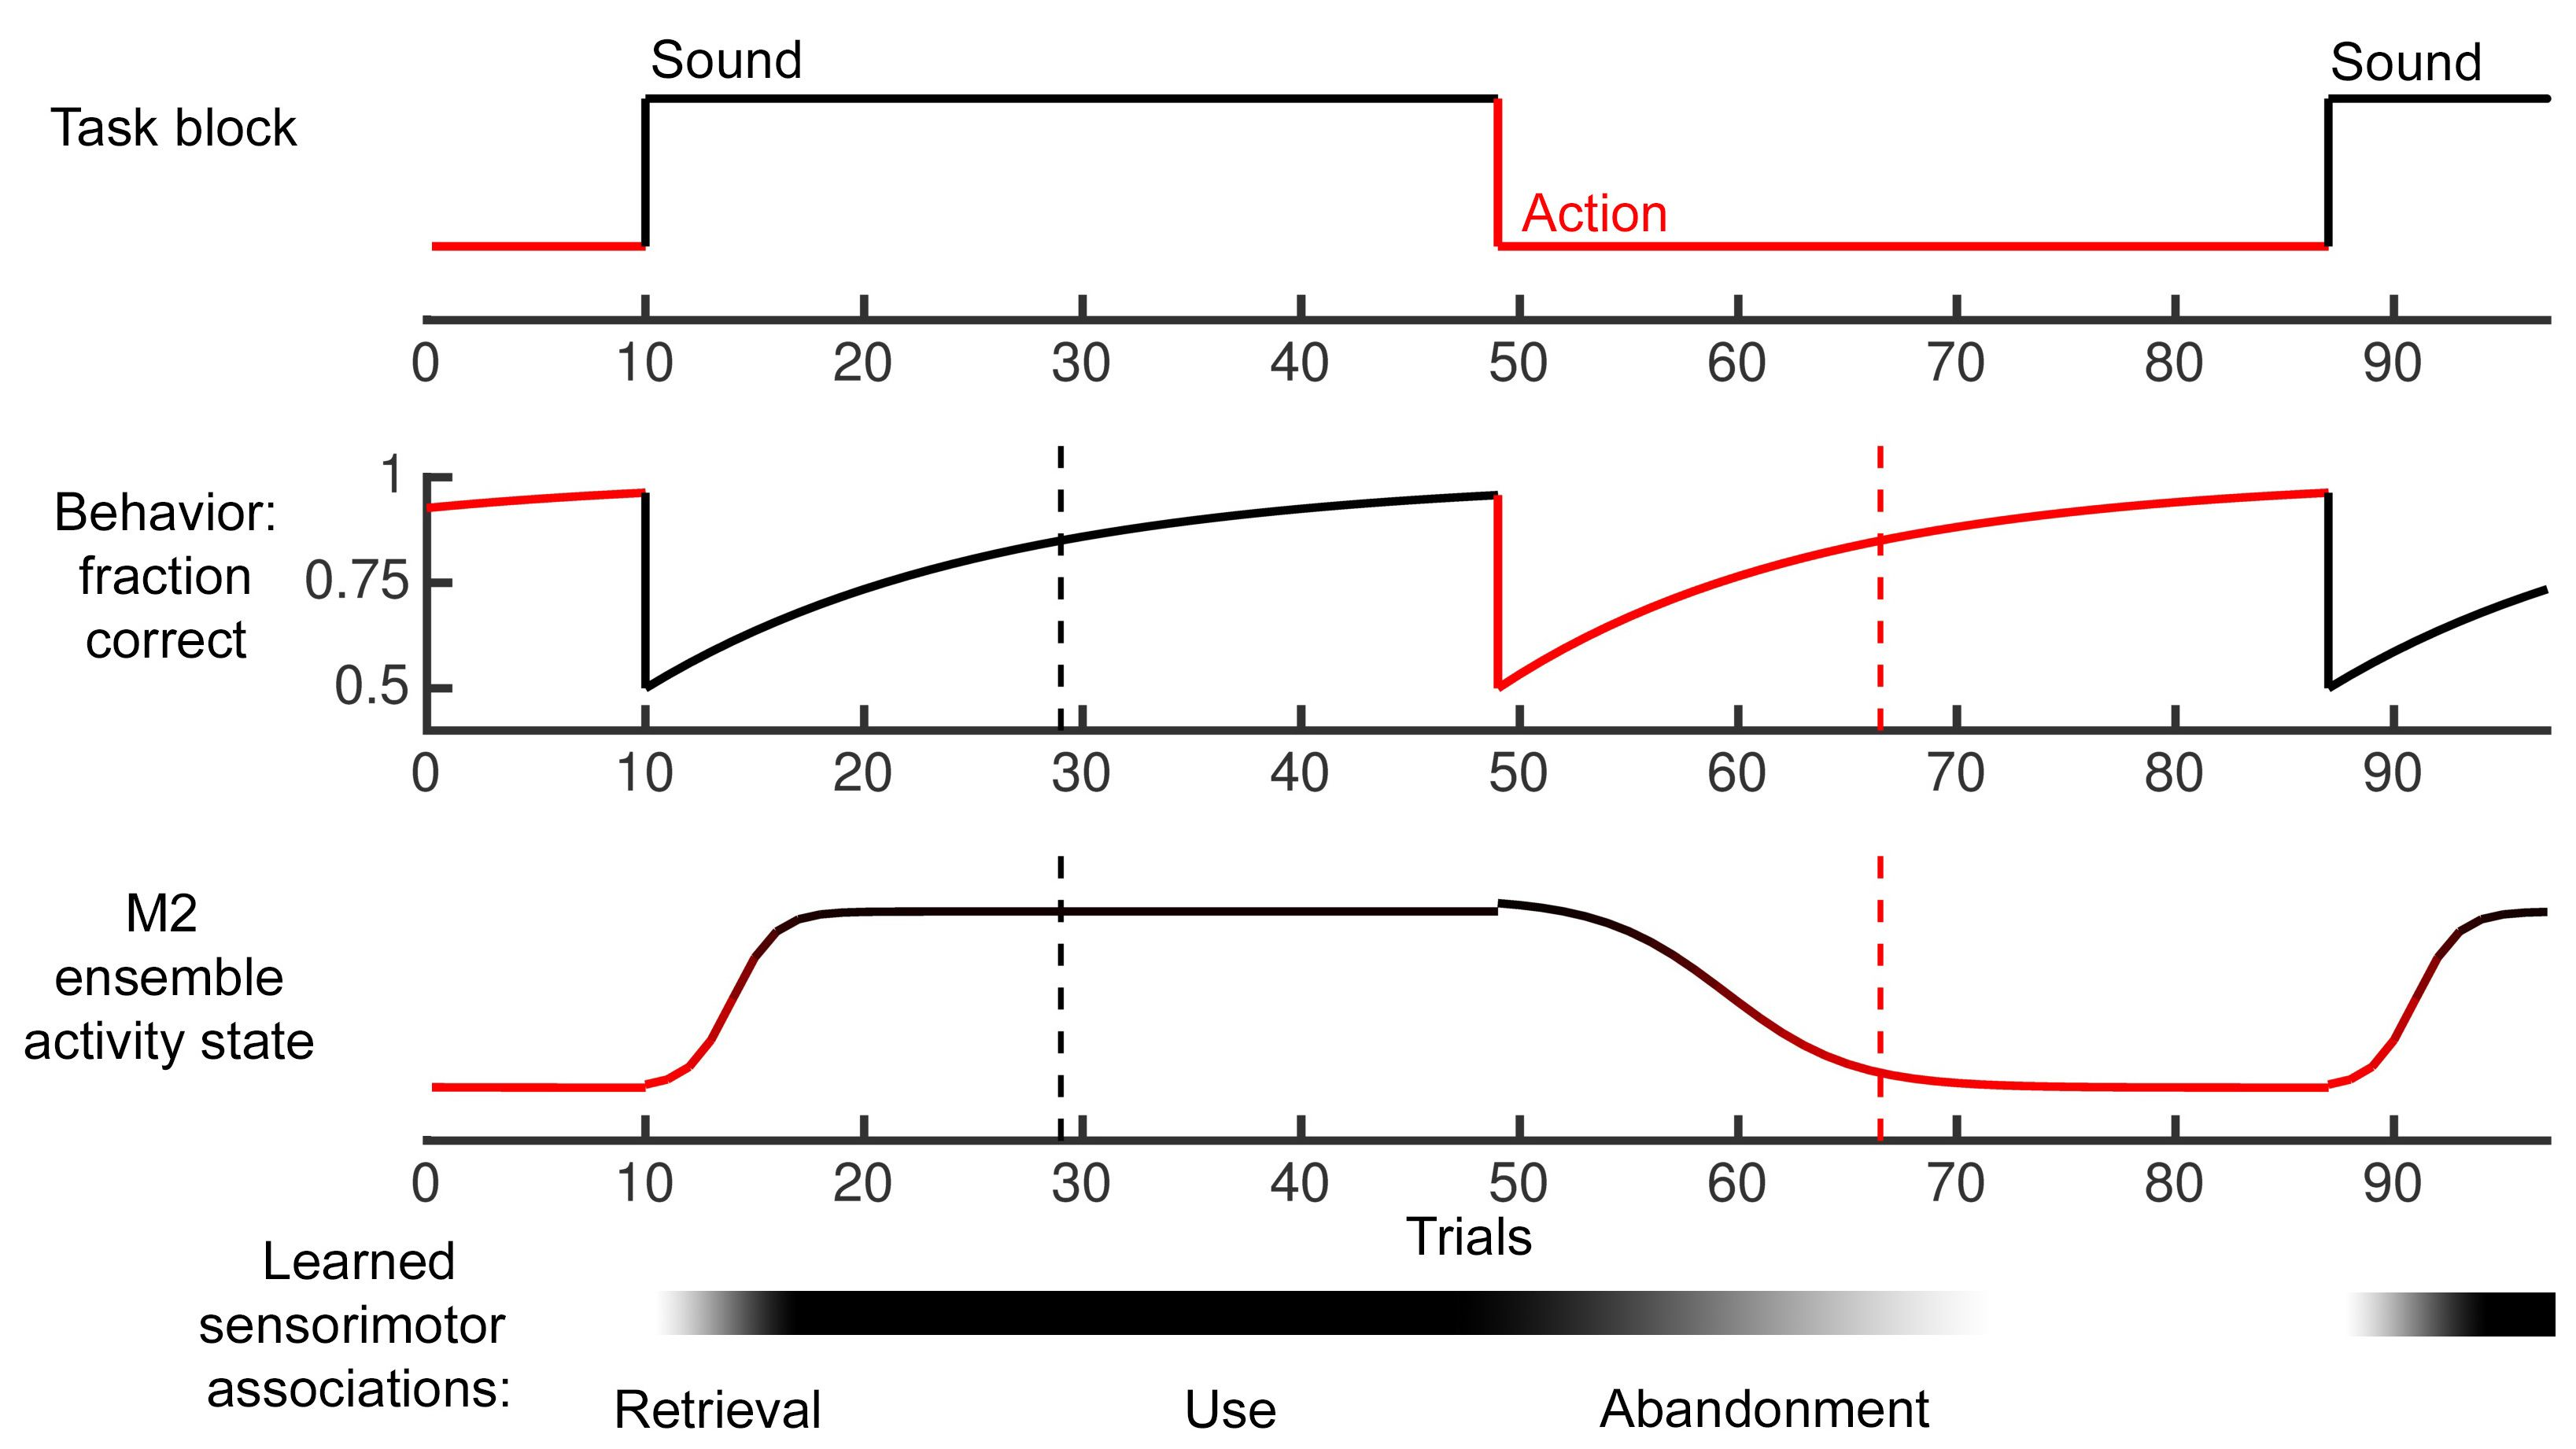
\includegraphics[width=\textwidth]{Figures/NN_figS9.jpg} 
\end{center}

\caption[Summary of the task, behavioral performance, and neural dynamics.]
{Summary of the task, behavioral performance, and neural dynamics. Recovery of behavioral performance following a rule switch (middle) was approximated as an exponential function for this schematic. Dashed lines reflect the median number of trials to a behavioral transition (sound: 19.0, action: 17.5) or neural transition (bottom; sound: 5.1, action: 14.6) relative to the rule switch. The plot of M2 ensemble activity state (bottom) was based on the midpoint trial (sound: 4.0, action: 10.4), steepness (sound: 1.02, action: 0.35), and range (sound: 0.36, action: 0.38) parameters estimated from logistic fits of the neural transition data (see Fig. \ref{fig:NN_fig4}).
}

\label{fig:NN_figS9}
\end{figure}